\documentclass[paper=a4, fontsize=11pt]{scrartcl} % A4 paper and 11pt font size

%----------------------------------------------------------------------------------------
%	PACKAGES
%----------------------------------------------------------------------------------------
\usepackage[T1]{fontenc} % Use 8-bit encoding that has 256 glyphs
\usepackage{fourier} % Use the Adobe Utopia font for the document - comment this line to return to the LaTeX default
\usepackage[english]{babel} % English language/hyphenation
\usepackage{amsmath,amsfonts,amsthm} % Math packages
\usepackage{sectsty} % Allows customizing section commands
\usepackage{fancyhdr} % Custom headers and footers
\usepackage{tabularx, outlines, framed, varwidth, enumitem, graphicx, listings, color, qtree, float, subcaption, newfloat}
\usepackage[left=0.5in, right=0.5in, top=3in, bottom=.25in]{geometry}
\geometry{}

%----------------------------------------------------------------------------------------
%	SET CUSTOMIZATIONS AND FUNCTIONS
%----------------------------------------------------------------------------------------
\sectionfont{\centering \normalfont\scshape} % Make all sections centered, the default font and small caps
\pagestyle{fancyplain} % Makes all pages in the document conform to the custom headers and footers
\fancyhead{} % No page header - if you want one, create it in the same way as the footers below
\fancyfoot[L]{} % Empty left footer
\fancyfoot[C]{} % Empty center footer
\fancyfoot[R]{\thepage} % Page numbering for right footer
\renewcommand{\headrulewidth}{0pt} % Remove header underlines
\renewcommand{\footrulewidth}{0pt} % Remove footer underlines
\setlength{\headheight}{0pt} % Customize the height of the header

\DeclareFloatingEnvironment[fileext=lod]{diagram}

\numberwithin{equation}{section} % Number equations within sections (i.e. 1.1, 1.2, 2.1, 2.2 instead of 1, 2, 3, 4)
\numberwithin{figure}{section} % Number figures within sections (i.e. 1.1, 1.2, 2.1, 2.2 instead of 1, 2, 3, 4)
\numberwithin{table}{section} % Number tables within sections (i.e. 1.1, 1.2, 2.1, 2.2 instead of 1, 2, 3, 4)

\graphicspath{{./figures/}}
%\setlength\parindent{0pt} % Removes all indentation from paragraphs - comment this line for an assignment with lots of text

\makeatletter
	\newcommand*\variableheghtrulefill[1][.4\p@]
	{%
		\leavevmode
		\leaders \hrule \@height #1\relax \hfill
		\null
	}
\makeatother

\lstset
{
	language=C++,
%	basicstyle=\ttfamily,
%	keywordstyle=\color{blue}\ttfamily,
%	stringstyle=\color{red}\ttfamily,
%	commentstyle=\color{green}\ttfamily,
%	morecomment=[l][\color{magenta}]{\#}
	keywordstyle=\color{blue},
	stringstyle=\color{red},
	commentstyle=\color{green},
	morecomment=[l][\color{magenta}]{\#}
}

%----------------------------------------------------------------------------------------
%	USEFUL COMMANDS
%----------------------------------------------------------------------------------------
%	\makebox[\textwidth][c]{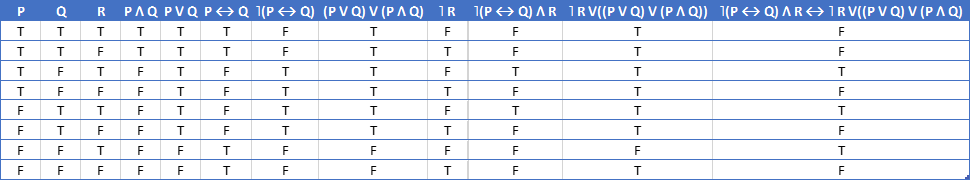
\includegraphics[width=.9\pagewidth]{p2-table}}

%	\newgeometry{top=.75in, bottom=.75in, left=.25in,right=.25in}
%	\newgeometry{top=.75in, bottom=.75in, left=1.25in,right=1.25in}

%	\lstinputlisting[firstline=4]{CMPSC360_Homework.cpp}

%\Tree
%	[.<root> [.<left> ][.<middle> ][.<right> ]]

%----------------------------------------------------------------------------------------
%	TITLE SECTION
%----------------------------------------------------------------------------------------

\newcommand{\horrule}[1]{\rule{\linewidth}{#1}} % Create horizontal rule command with 1 argument of height
% \title{Template: Homework 1}
\title{	
\normalfont \normalsize 
%\textsc{Rutgers University, Real Analysis I} \\ [25pt] % Your university, school and/or department name(s)
\horrule{0.5pt} \\[0.4cm] % Thin top horizontal rule
\huge STAT 463: Homework 6 \\ % The assignment title
\horrule{2pt} \\[0.5cm] % Thick bottom horizontal rule
}

\author{\textbf{\underline{Name:}}Kyle Salitrik | \textit{\textbf{\underline{ID\#:}} 997543474} | \textit{\textbf{\underline{PSU ID:}} kps168}} % Your name

\date{\normalsize\today} % Today's date or a custom date

\begin{document}

\maketitle % Print the title
\newgeometry{top=.75in, bottom=.75in, left=1.25in,right=1.25in}

%----------------------------------------------------------------------------------------
%	PROBLEM 1
%----------------------------------------------------------------------------------------



\section*{\variableheghtrulefill[.25ex]\quad Problem 1 \quad\variableheghtrulefill[.25ex]}
\subsection*{a)}
\lstinputlisting[language=]{listings/p1_additive_seasonal.txt}

\subsection*{b)}
From part A we see that the seasonal component in october is 95.226620, therefore we estimate: $735 - 95.226620 = 639.7734$

\subsection*{c)}
\makebox[\textwidth][c]{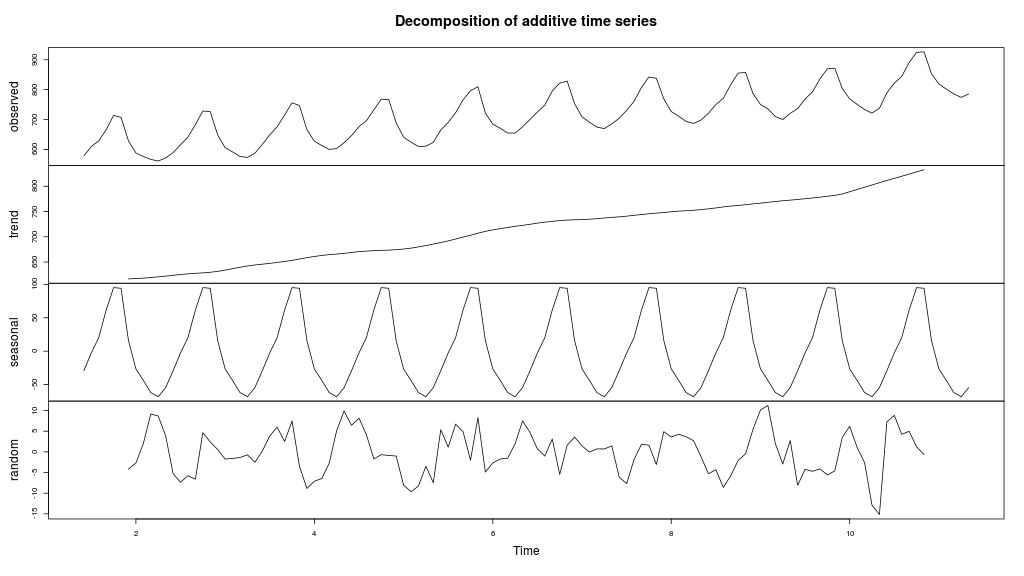
\includegraphics[scale=.5]{p1_part_c.png}}

\subsection*{d)}
\lstinputlisting[language=]{listings/p1_multiplicative_seasonal.txt}

\subsection*{e)}
Again, using the values from part D: $735 - 1.1335675 = 733.8664$

\subsection*{f)}
\lstinputlisting[language=]{listings/p1_lowess_effects.txt}

\subsection*{g)}
Yes, the trend is linear, not exponential or polynomial so the additive decomposition is suitable.

%----------------------------------------------------------------------------------------
%	PROBLEM 2
%----------------------------------------------------------------------------------------

\section*{\variableheghtrulefill[.25ex]\quad Problem 2 \quad\variableheghtrulefill[.25ex]}
\subsection*{a)}
Looking at the ACF and plots of the raw data, there appears to be a seasonality and linear trend to the dataset.

\makebox[\textwidth][c]{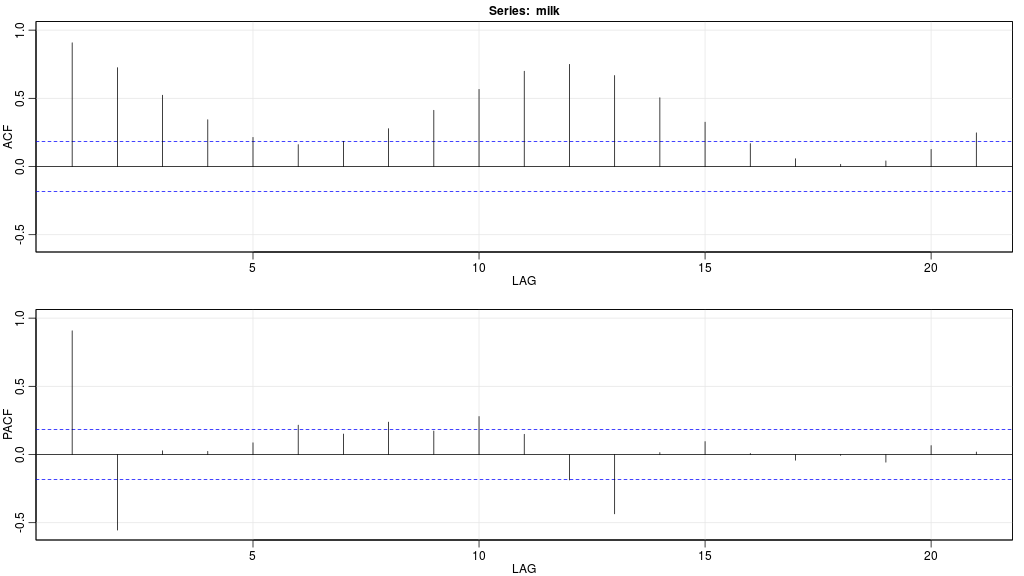
\includegraphics[scale=.5]{p2_part_a_1.png}}

Because of these trends, a first difference was made for all of the data followed by a seasonal difference of 12 months. The result is the following ACF plot:

\makebox[\textwidth][c]{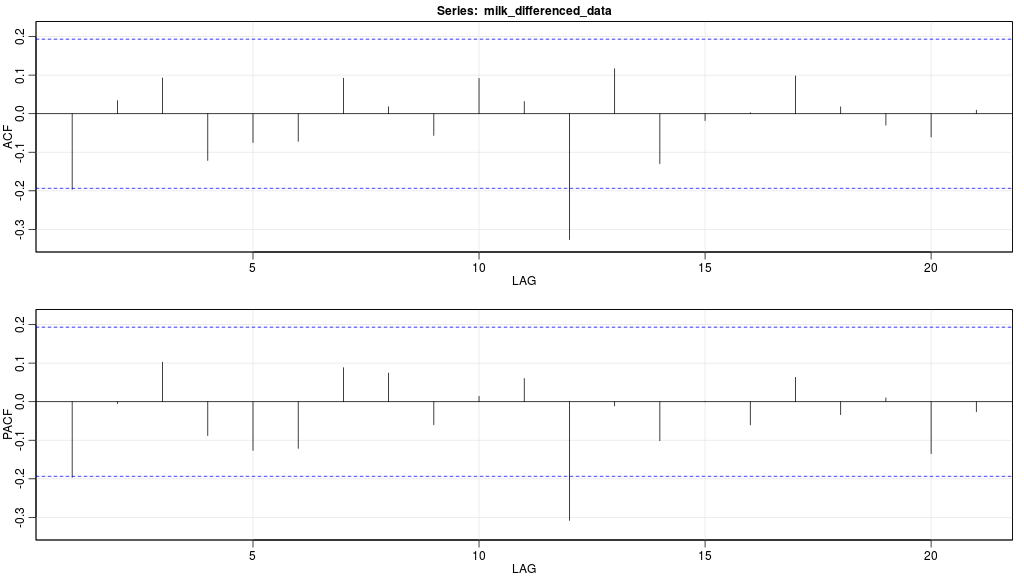
\includegraphics[scale=.5]{p2_part_a_2.png}}

\subsection*{b)}
Based on the above ACF and PACF plots, a SARIMA model of (1,1,1)(1,1,1)[12] was used. This model is potentially valuable because there is a single spike in the early lags of both the PACF and ACF, followed by a significant spike after 12 months and no others.

\makebox[\textwidth][c]{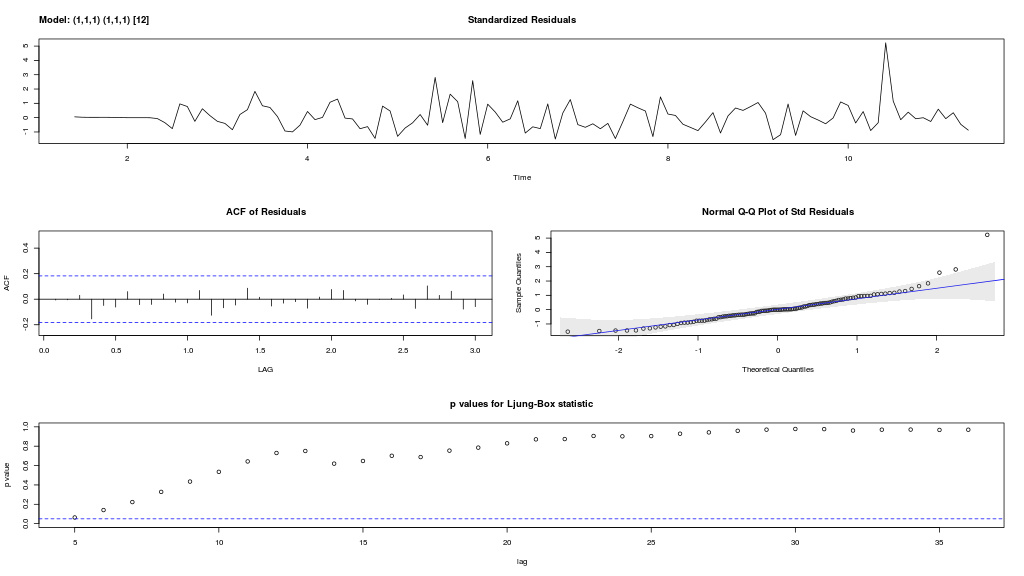
\includegraphics[scale=.5]{p2_part_b.png}}

\subsection*{c)}
\lstinputlisting[language=]{listings/p2_predictions.txt}

\makebox[\textwidth][c]{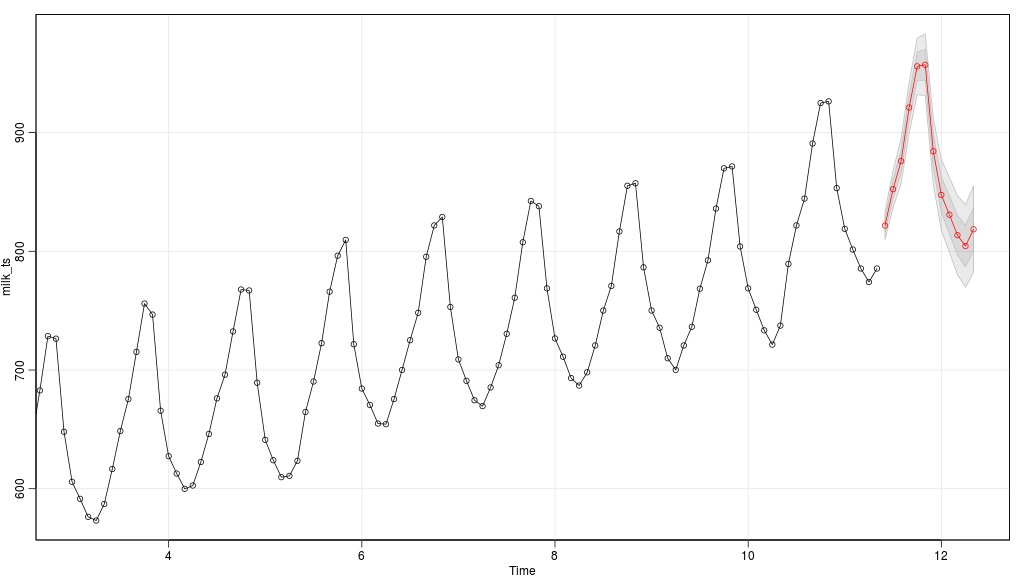
\includegraphics[scale=.5]{p2_part_c.png}}



%----------------------------------------------------------------------------------------
%	PROBLEM 3
%----------------------------------------------------------------------------------------

\section*{\variableheghtrulefill[.25ex]\quad Problem 3 \quad\variableheghtrulefill[.25ex]}
\subsection*{a)}
Plotting the data and observing the trends shows that there is possibly a quarterly or 4-month trend as well as a possible 5 year trend, although there is not enough future data to prove this. Using a set of weights of $\{\frac{1}{8}, \frac{1}{4}, \frac{1}{4}, \frac{1}{4}, \frac{1}{8}\}$ found through trial and error, the following plot was obtained:

\makebox[\textwidth][c]{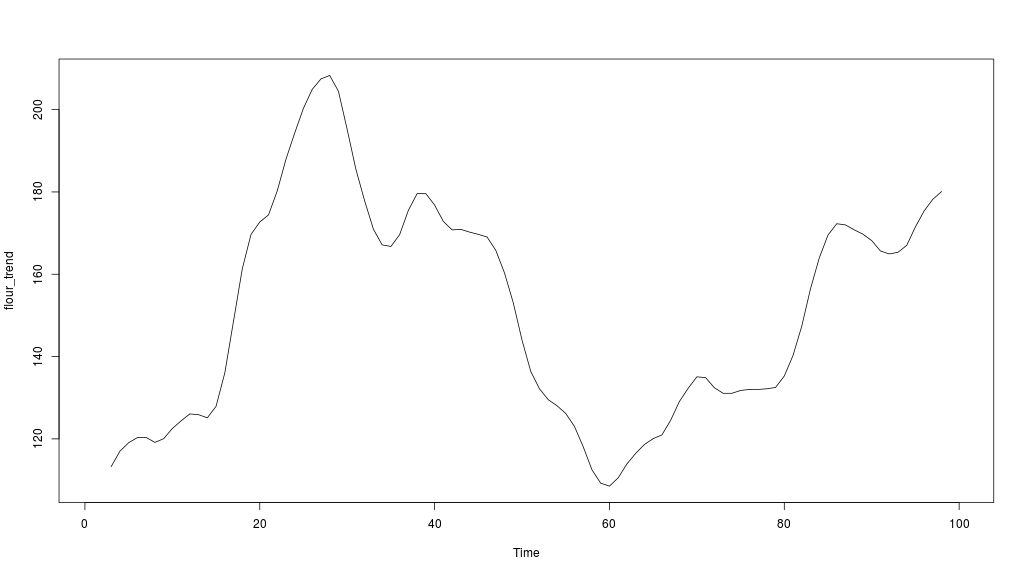
\includegraphics[scale=.5]{p3_part_a.png}}

\subsection*{b)}
\makebox[\textwidth][c]{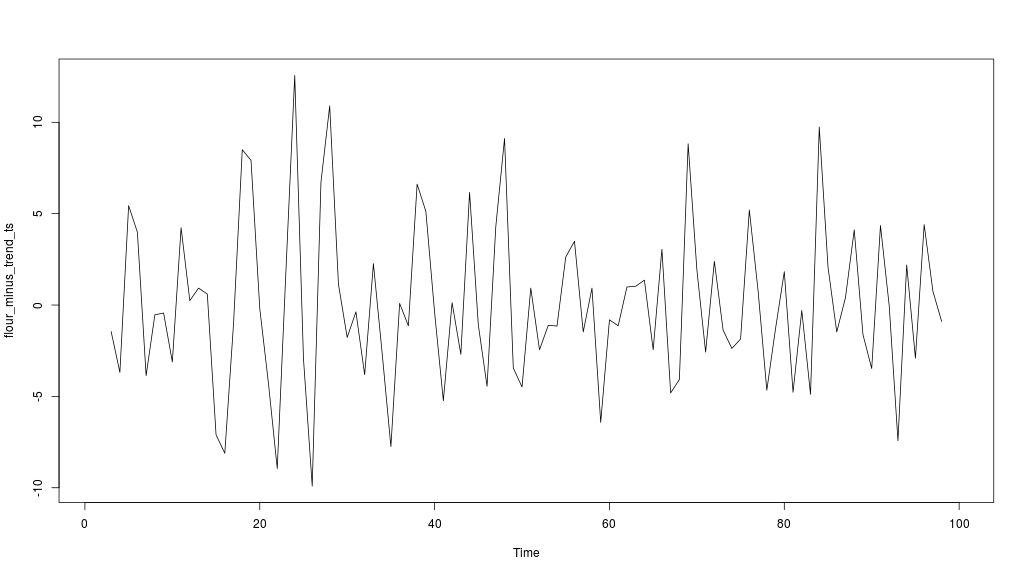
\includegraphics[scale=.5]{p3_part_b.png}}

\subsection*{c)}
\makebox[\textwidth][c]{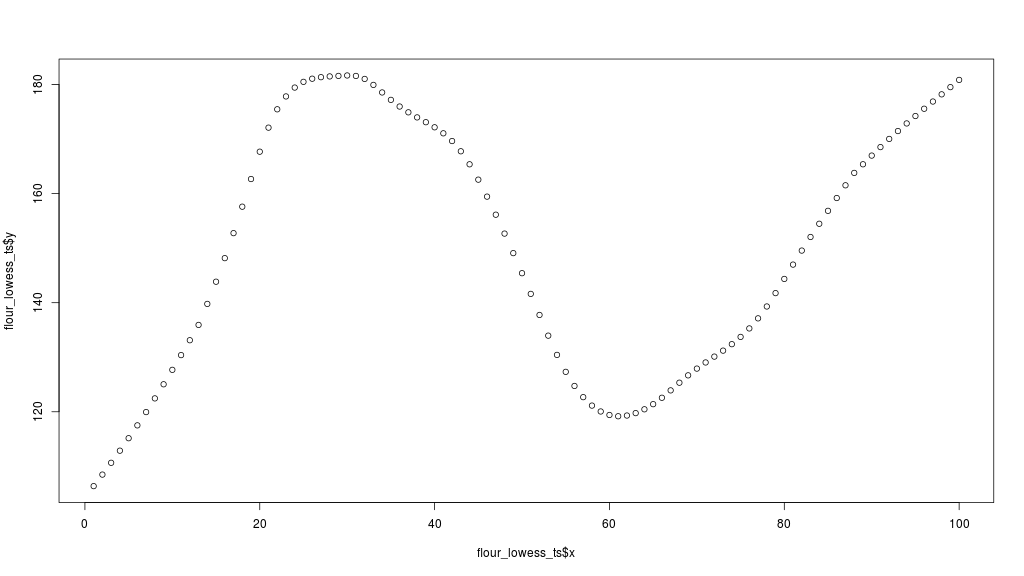
\includegraphics[scale=.5]{p3_part_c.png}}

\subsection*{d)}
As f increases, the plot approaches a straight line at the mean

\makebox[\textwidth][c]{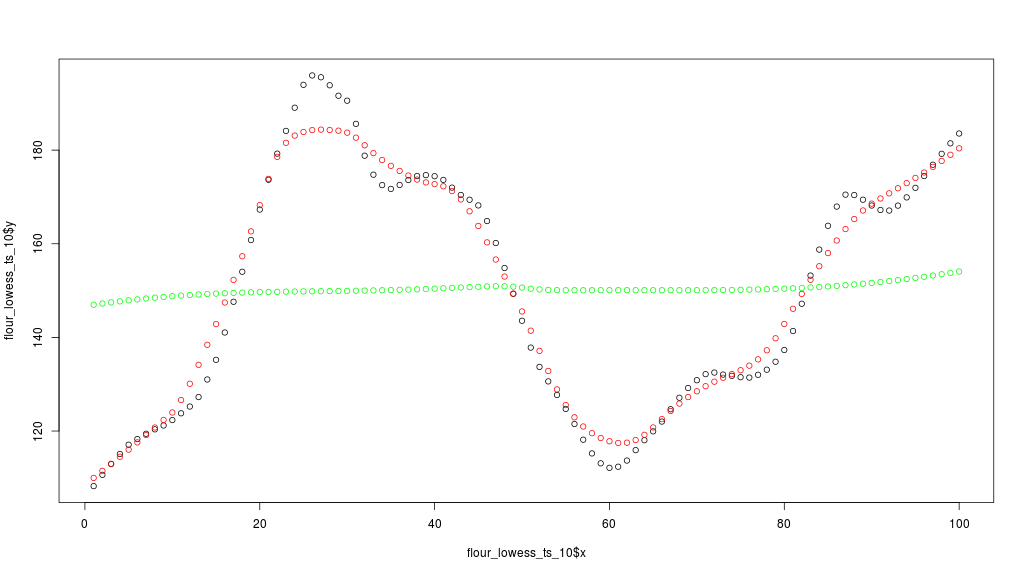
\includegraphics[scale=.5]{p3_part_d.png}}

\subsection*{e)}
The MA coefficient is $0.2891139$ and the alpha value is $1.2891139$

\subsection*{f)}
\makebox[\textwidth][c]{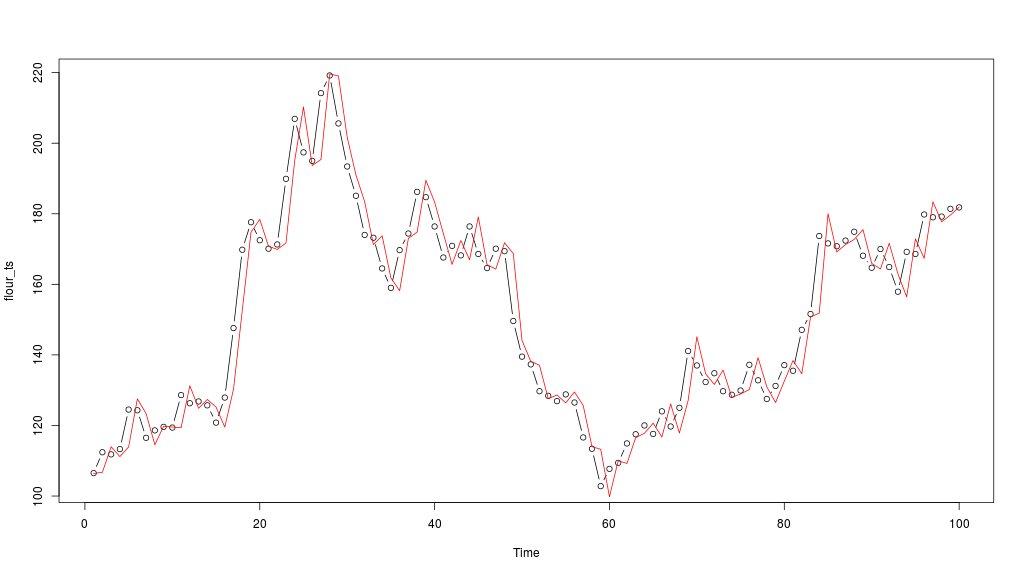
\includegraphics[scale=.5]{p3_part_f.png}}

\subsection*{g)}
The prediction for $t = 101$ is $(1.2891139 * 181.8) - (0.2891139 * 181.8) = 181.7673$

\end{document}